\chapter{现金流量的构成}
\noindent \textbf{本章知识点:}\\
1.\textbf{现金流入、现金流出}、净现金流量的概念\\
2.\textbf{建设投资}的概念、构成,\textbf{对现金流的影响}\\
3.固定资产、无形资产、其他资产的概念\\
4.固定资产的原值、\textbf{折旧、净残值,折旧对现金流的影响}\\
5.固定资产折旧的方法:\textbf{直线折旧}法、工作量法\\
6.无形资产的\textbf{摊销}\\
7.流动资金投资及其特点、\textbf{对现金流的影响}\\
8.总成本费用的构成\\
9.\textbf{机会成本、沉没成本}\\
10.\textbf{总成本费用和经营成本的区别、联系};二者对现金流的影响\\
11.了解增值税、消费税、企业所得税对现金流的影响\\
12.\textbf{收入、成本、税金和利润的关系}\\
13.区分\textbf{初始现金流、营业现金流及终结现金流}\\
\textbf{注意:加粗部分为期末考试重点内容。}

\section{基本概念}

\subsection{投资}

广义概念:人们的一种有目的的经济行为,即以一定的资源投入某项计划,以获取所期望的报酬。

狭义概念:人们在社会经济活动中为实现某种预定的生产目标而预先垫支的资金。

本课程常用的投资是投资的狭义概念。

包括:\textbf{固定资产投资、流动资金投资、无形资产投资、递延资产投资和预备费用、(建设期利息)}。

固定资产投资活动按其工作内容和实现方式分为:“建筑安装工程”;“设备、工具、器具购置”;“其他费用”三个部分。

\begin{figure}[H]
    \centering
    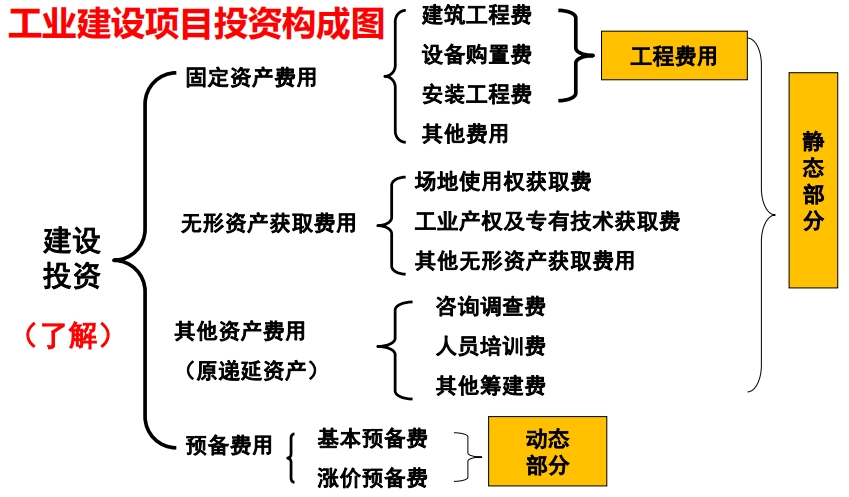
\includegraphics[width=\textwidth]{image/投资分类.png}
    \caption{工业建设项目投资构成图}
\end{figure}

\subsection{现金流量(Cash Flow)}
工业生产活动考察两个方面:物质形态(工具、设备、能耗产品)与货币形态(资金投入、成本收入)。技术经济分析中,把各时点上实际发生的以货币形式体现的资金流出或资金流入称为现金流量。

\subsection{现金流出}
对一个系统而言,凡在某一时点上流出系统的资金或货币量,如投资、费用等。流出系统的现金称为现金流出。(CO)

\subsection{现金流入}
对一个系统而言,凡在某一时点上流入系统的资金或货币量,如销售收入等。流入系统的现金称为现金流入。(CI)

$$
\mbox{净现金流量(}NCF\mbox{)}=\mbox{现金流入(}CI\mbox{)}-\mbox{现金流出(}CO\mbox{)}
$$

现金流量确定原则:收付实现制(实付实收);

会计记账原则:权责发生制(应付应收)。

现金流比会计利润更能反映投资收益,现金流分析是投资决策分析的基础,若现金流预测不准确,无论投资决策分析多准确,都将导致错误的决策。

现金流为投资决策提供重要的价值信息;现金流更有利于考虑资金的时间价值,而会计利润不考虑资金收付时间。

现金流有助于了解收益质量、取得和运用现金的能力,支付本息和股利的能力,同时提供了信用基础。

构成现金流量的基本因素有:成本、投资、税金、利润、收入。\textbf{(往年期中考题)}

\section{各种资产分类}
\subsection{固定资产}
固定资产界定(考点,会考选择题/判断题):

企业为生产商品、提供劳务、出租或经营管理而持有的;\textbf{使用年限超过一个会计年度单位价值较高,并在使用过程中保持原有实物形态的资产}。包括房屋、建筑物、机器、设备等。

\textbf{使用年限要长,单位价值要高,使用过程中要保持原有实物形态的资产(比如煤炭,烧完了就没了,就不算固定资产)。}

\textbf{考固定资产和流动资金的对比或固定资产的三要素。}

以下内容来自百度,但我觉得只要回答出固定资产三要素就可以了,因为这三要素是固定资产的特点:

流动资产是指可以在1年或者超过1年的一个经营周期内变现或者耗用的资产。流动资产投资是指工程在投产前预先垫付、在投产后生产经营过程中周转使用的资金。主要区别为:

〔1〕固定资产投资的结果形成劳动手段,流动资产投资的结果是劳动对象,流动资产投资的数量是由固定资产投资的规模及其结构所决定的。

〔2〕固定资产和流动资产都是生产不可缺少的生产要素,固定资产投资必须有流动资产投资的配合。

〔3〕固定资产投资从工程开工到建成交付使用,往往要经历很长的时间,只有投入没有产出。固定资产投资时间短,回收快。

〔4〕固定资产价值的回收依赖于流动资产的顺利周转。

固定资产计价:原始价值、折旧、净值、重估值、净残值。以下内容将是期末计算题第一题考点:

\subsubsection{固定资产原始价值(原值)}
企业为取得某项固定资产所支付的\textbf{全部价款(包括利息等)}以及使固定资产达到预计可使用状态前所发生的一切合理、必要的支出。包括固定资产费用、固定资产投资借款建设期利息、预备费。

\subsubsection{固定资产折旧}
工业项目投入运营之后,固定资产在使用过程中会逐渐磨损和贬值,其价值逐步转移到产品中去,伴随固定资产损耗发生的价值转移称为折旧。

\subsubsection{固定资产净值}
固定资产使用一段时间后,其原值扣除累计的折旧费总额。
$$\mbox{固定资产原值}-\mbox{累计折旧}=\mbox{固定资产净值}$$

\subsubsection{重估值(重置成本)}
对固定资产按照社会再生产条件和市场情况进行的价值的重新评估。即在当前的生产技术条件下,以现行价格水平重新购建\textbf{同样全新的固定资产}所需要的全部支出。

\subsubsection{预计净残值}
假定固定资产预计使用寿命已满并处于使用\textbf{寿命终了时的预期状态},企业从该项资产的处置中获得的扣除预计处置费用后的金额。

\textbf{折旧是每年都有的,净残值是只有设备最后一年才有的。}
$$\mbox{预计净残值}=\mbox{处置收入}-\mbox{处置费用}$$
或
$$\mbox{预计净残值}=\mbox{固定资产原值} \times \mbox{净残值率}$$
它是固定资产处置时可在市场上实现的价值,对于工业项目的投资者来说,是一项\textbf{在期末可回收的现金流入}。

\noindent \textbf{判断题:}固定资产的残值回收可作为项目的一项现金流入。\\
\textbf{答案:正确}。

\noindent (多选题)下面哪些影响固定资产年折旧额大小?\\
A.固定资产原值大小\\
B.净残值\\
C.折旧年限\\
\textbf{答案:ABC}

这里不讲折旧的计算,在把各种资产分类讲完后统一介绍。

\subsection{流动资产投资}
会计上称为营运资金,营运资本。指在工业项目投产前预先垫付,在投产后的生产经营过程中用于购买原材料、燃料动力,备品备件,支付工资和其他费用,以及在在产品、半成品,产成品和其他存货占用的\textbf{周转资金}。

特点:整个项目寿命期内,流动资金始终被占用且周而复始地流动,到\textbf{项目寿命期结束时},全部流动资金退出生产和流通,以货币资金形式\textbf{回收(现金流入)}。

投产第一年所需的流动资金应在项目投产前安排,为简化计算,项目评价时流动资金可从\textbf{投产第一年}开始安排(\textbf{现金流出})。

储备资金(原材料、燃料等)、生产资金(在制品、半成品、待摊费用)、成品资金(产成品、外购品等)、结算资金(应收、预付帐款等)、货币资金(备用金、现金、银行存款等)。\\
例:(多选)关于流动资金,说法正确的是\\
A.当发生流动资金投资时,应计入现金流出\\
B.一般当寿命期结束时,流动资金作为现金流入\\
C.一般当寿命期结束时,流动资金作为现金流出\\
答案:AB。

\subsection{无形资产}
界定:企业拥有或者控制的没有实物形态的可辨认非货币性资产。如:包括专利、著作权、版权、商标、专有技术、非专利技术、特许权等;其价值在服务期内逐年摊销,摊销费计入成本。

无形资产原值——无形资产购建费用、无形资产投资建设期借款利息;

无形资产的摊销——无形资产的价值在服务期内通过摊销(直线法)的形式计入费用。

\subsection{递延资产}
递延资产,是指本身没有交换价值,不可转让,一经发生就已消耗,但能为企业创造未来收益,并能从未来收益的会计期间抵补的各项支出。包括开办费、租赁固定资产改良费、固定资产装璜、装修费等中在规定年限内平均摊销,摊销费计入成本。

界定:在项目筹建期内实际发生的各项费用,除应计入固定资产和无形资产外的,均计入其他资产(递延资产)。如生产准备费、办公及生活家具购置费等开办费性质的费用直接形成其他资产。

其他资产摊销费——其他资产应在项目投入运营后的一定年限内平均摊销,摊销费计入费用。\\
例1:(多选)建设投资形成的资产包括\\
A.固定资产\\
B.无形资产\\
C.建设期利息\\
D.其他资产\\
答案:ABD。\\
例2:(单选)项目财务评价中确定现金流量的基本原则是\\
A.权责发生制\\
B.收付实现制\\
答案:B。\\
例3:(判断)流动资金投资,当发生时是现金流出,此说法\\
答案:正确。


\section{折旧的计算}
\noindent \textbf{固定资产的折旧方法:}

直线法(年限平均法)

工作量法

双倍余额递减法

年数总和法

\subsection{直线法(使用最广泛)}
$$\mbox{年折旧额}=\mbox{(原值}-\mbox{净残值)}/\mbox{折旧年限}$$
或
$$\mbox{年折旧额}=\mbox{固定资产原值} \times \mbox{年折旧率}$$
$$\mbox{年折旧率}=(1-\mbox{净残值率})/\mbox{折旧年限}×100\%$$

例题1:某固定资产原值为1万元,预计净残值率为4\%,折旧年限为5年,则按平均年限法计算年折旧率、年折旧额及第3年末帐面净值分别为多少?

解:$f=\frac{1-4\%}{5} \times 100\% = 19.2\%$

$D=10000 \times 19.2\%=1920$(元)

$K_3=10000-1920 \times 3=4240$(元)


\subsection{工作量法}
(1)计算公式
$$\mbox{单位工作量折旧额=(固定资产原值-净残值)/预计使用年限内可完成的工作量}$$
$$\mbox{年折旧额=单位工作量折旧额} \times \mbox{年实际完成的工作量}$$
(2)特点

使用年限内每年的单位折旧额不变,年折旧额随年实际工作量而变化。

(3)适用-某些专业设备、交通运输车辆等。

例题2:计算一台估计生产10万个单位的设备折旧额。设备成本为1万元,预计前两年每年生产2万个单位,第三年生产3万个单位,第四年生产1万个单位,最后一年生产2万个单位。

解:不给净残值时,净残值默认为0。

单位产量折旧额$=(10000-0)/100000=0.1$(元)

第一年折旧额$=0.1 \times 20000 = 2000$(元)

第二年折旧额$=0.1 \times 20000 = 2000$(元)

第三年折旧额$=0.1 \times 30000 = 3000$(元)

第四年折旧额$=0.1 \times 10000 = 1000$(元)

第五年折旧额$=0.1 \times 20000 = 2000$(元)

\subsection{双倍余额递减法}
(1)含义(看不懂就去看公式和例题)

在寿命期 1 到(n - 2)年,不考虑固定资产残值的情况下,根据每期期初固定资产账面净值和双倍的直线法折旧率计算固定资产折旧。

在寿命期的最后两年,将第 n - 1 年年初的固定资产账面净值扣除净残值后的余额进行平摊。

\textbf{刚开始折旧多,后面折旧少。前期可以少交税。}

(2)计算公式(记住就行)

1 到 n - 2 年:
$$\mbox{年折旧率=}2 / \mbox{折旧年限} \times 100\%$$
$$\mbox{年折旧额=每年年初固定资产账面净值} \times \mbox{年折旧率}$$
第 n - 1 年、第 n 年:
$$\mbox{第 n - 1 年年初固定资产账面净值-净残值} /2$$

例题3:仍以例题1数据为例,双倍余额递减法的年折旧率$=2/5=0.4$,各年折旧额及年末帐面净值如下表所示(从第四年起改为直线折旧)。
\begin{table}[H]
\centering
\caption{双倍余额递减法折旧计算表}
\begin{tabular}{cccc}
\toprule
使用年限 & 年折旧率 & 年折旧额(元) & 年末净值(元) \\
\midrule
0 & 0 & 0 & 10000 \\
1 & 0.4 & 4000 & 6000 \\
2 & 0.4 & 2400 & 3600 \\
3 & 0.4 & 1440 & 2160 \\
4 &  & 880 & 1280 \\
5 &  & 880 & 400 \\
\bottomrule
\end{tabular}
\end{table}

\subsection{年数总和法}
(1)计算公式(了解一下吧,感觉不会考)
$$\mbox{年折旧率}=\frac{(\mbox{折旧年限}-\mbox{已使用年限)}}{[\mbox{折旧年限} \times (\mbox{折旧年限}+1)\div 2]}$$
$$\mbox{年折旧额}=(\mbox{原值}-\mbox{净残值}) \times \mbox{当年折旧率}$$
其中,折旧年限指预计总使用年限,已使用年限按照每年年初算;净残值计算时,每年计提折旧的基数不变,但是乘当年折旧率时,每年折旧率减少。

(2)特点

年折旧率和年折旧额都逐年减少,前期可以少交税。

例题4:仍以例题1数据为例,按年数总和法计算的各年折旧率、年折旧额及年末帐面净值如下表所示。
\begin{table}[H]
\centering
\caption{年数总和法折旧计算表}
\begin{tabular}{cccc}
\toprule
使用年限 & 年折旧率 & 年折旧额(元) & 年末净值(元) \\
\midrule
0 & 0 & 0 & 10000 \\
1 & 5/15 & 3200 & 6800 \\
2 & 4/15 & 2560 & 4240 \\
3 & 3/15 & 1920 & 2320 \\
4 & 2/15 & 1280 & 1040 \\
5 & 1/15 & 640 & 400 \\
\bottomrule
\end{tabular}
\end{table}

\subsection{总结}
注意:这里的点可能会考选择题,最后一点可考计算。

采用不同的折旧方法,对同一资产来说,计提的\textbf{折旧总额是相同的},只是每年计提的折旧数额不同;

无形资产、其他资产(原递延资产)的摊销与固定资产折旧的性质相同,均是把固定资产、无形资产、其他资产(原递延资产)的原始价值在一定期限内采用一定的人为方法进行分摊。

计提的折旧数额、摊销数额均计入产品成本或当期费用,即固定资产、无形资产、递延资产的价值通过计提折旧、摊销的方式转移到产品成本中,或转化为当期的费用。

在进行现金流量分析时,\textbf{计提折旧与摊销既不发生现金的流入,也没有发生现金流出},但因其\textbf{计入了成本费用},因而会\textbf{影响当期的利润数额}。

折旧和摊销虽然不是现金流入和流出,但是因为它影响了利润,所以会进而影响到税金。

\noindent \textbf{自测题(不要翻看前面的内容,直接作答):}

\noindent 1. (单选)对同一资产来说,采用不同的折旧方法:\\
A. 计提的折旧总额是相同的,只是每年计提的折旧数额不同。\\
B. 计提的折旧总额不相同的,每年计提的折旧数额也不同。\\
C. 计提的折旧总额是相同的,每年计提的折旧数额也相同。\\
D. 计提的折旧总额是不同的,每年计提的折旧数额相同。

\noindent 2. (单选)在进行现金流量分析时,计提折旧与摊销:\\
A. 不发生现金的流入,但会发生现金流出。\\
B. 发生现金的流入,但不发生现金流出。\\
C. 既不发生现金的流入,也不发生现金流出。\\
D. 既发生现金的流入,也发生现金流出。

\noindent 3. (单选)关于折旧,说法正确的是\\
A. 折旧不影响成本费用的大小\\
B. 折旧不影响现金流量\\
C. 折旧有的时候是现金流出\\
D. 折旧总额的大小不受折旧年限的影响\\
\textbf{答案:A、C、D。}

\section{费用、成本}
\subsection{概念解释}
费用:企业在生产经营过程中发生的各项耗费。(针对一定时间期间)

成本:企业为生产产品和提供劳务所发生的各项费用。(针对产品或劳务)

总成本费用:指项目在一定时期内(一般为一年)为生产和销售产品而花费的全部成本和费用。
\subsection{成本的分类}
成本计算范围:总成本费用、单位产品成本。

财务评价要求:总成本费用、经营成本。

成本与产量:固定成本、可变成本。

其他方式:机会成本、资金成本等。

\subsection{总成本费用的构成——按经济用途分类(看看,有个印象就行)}
\begin{figure}[H]
    \centering
    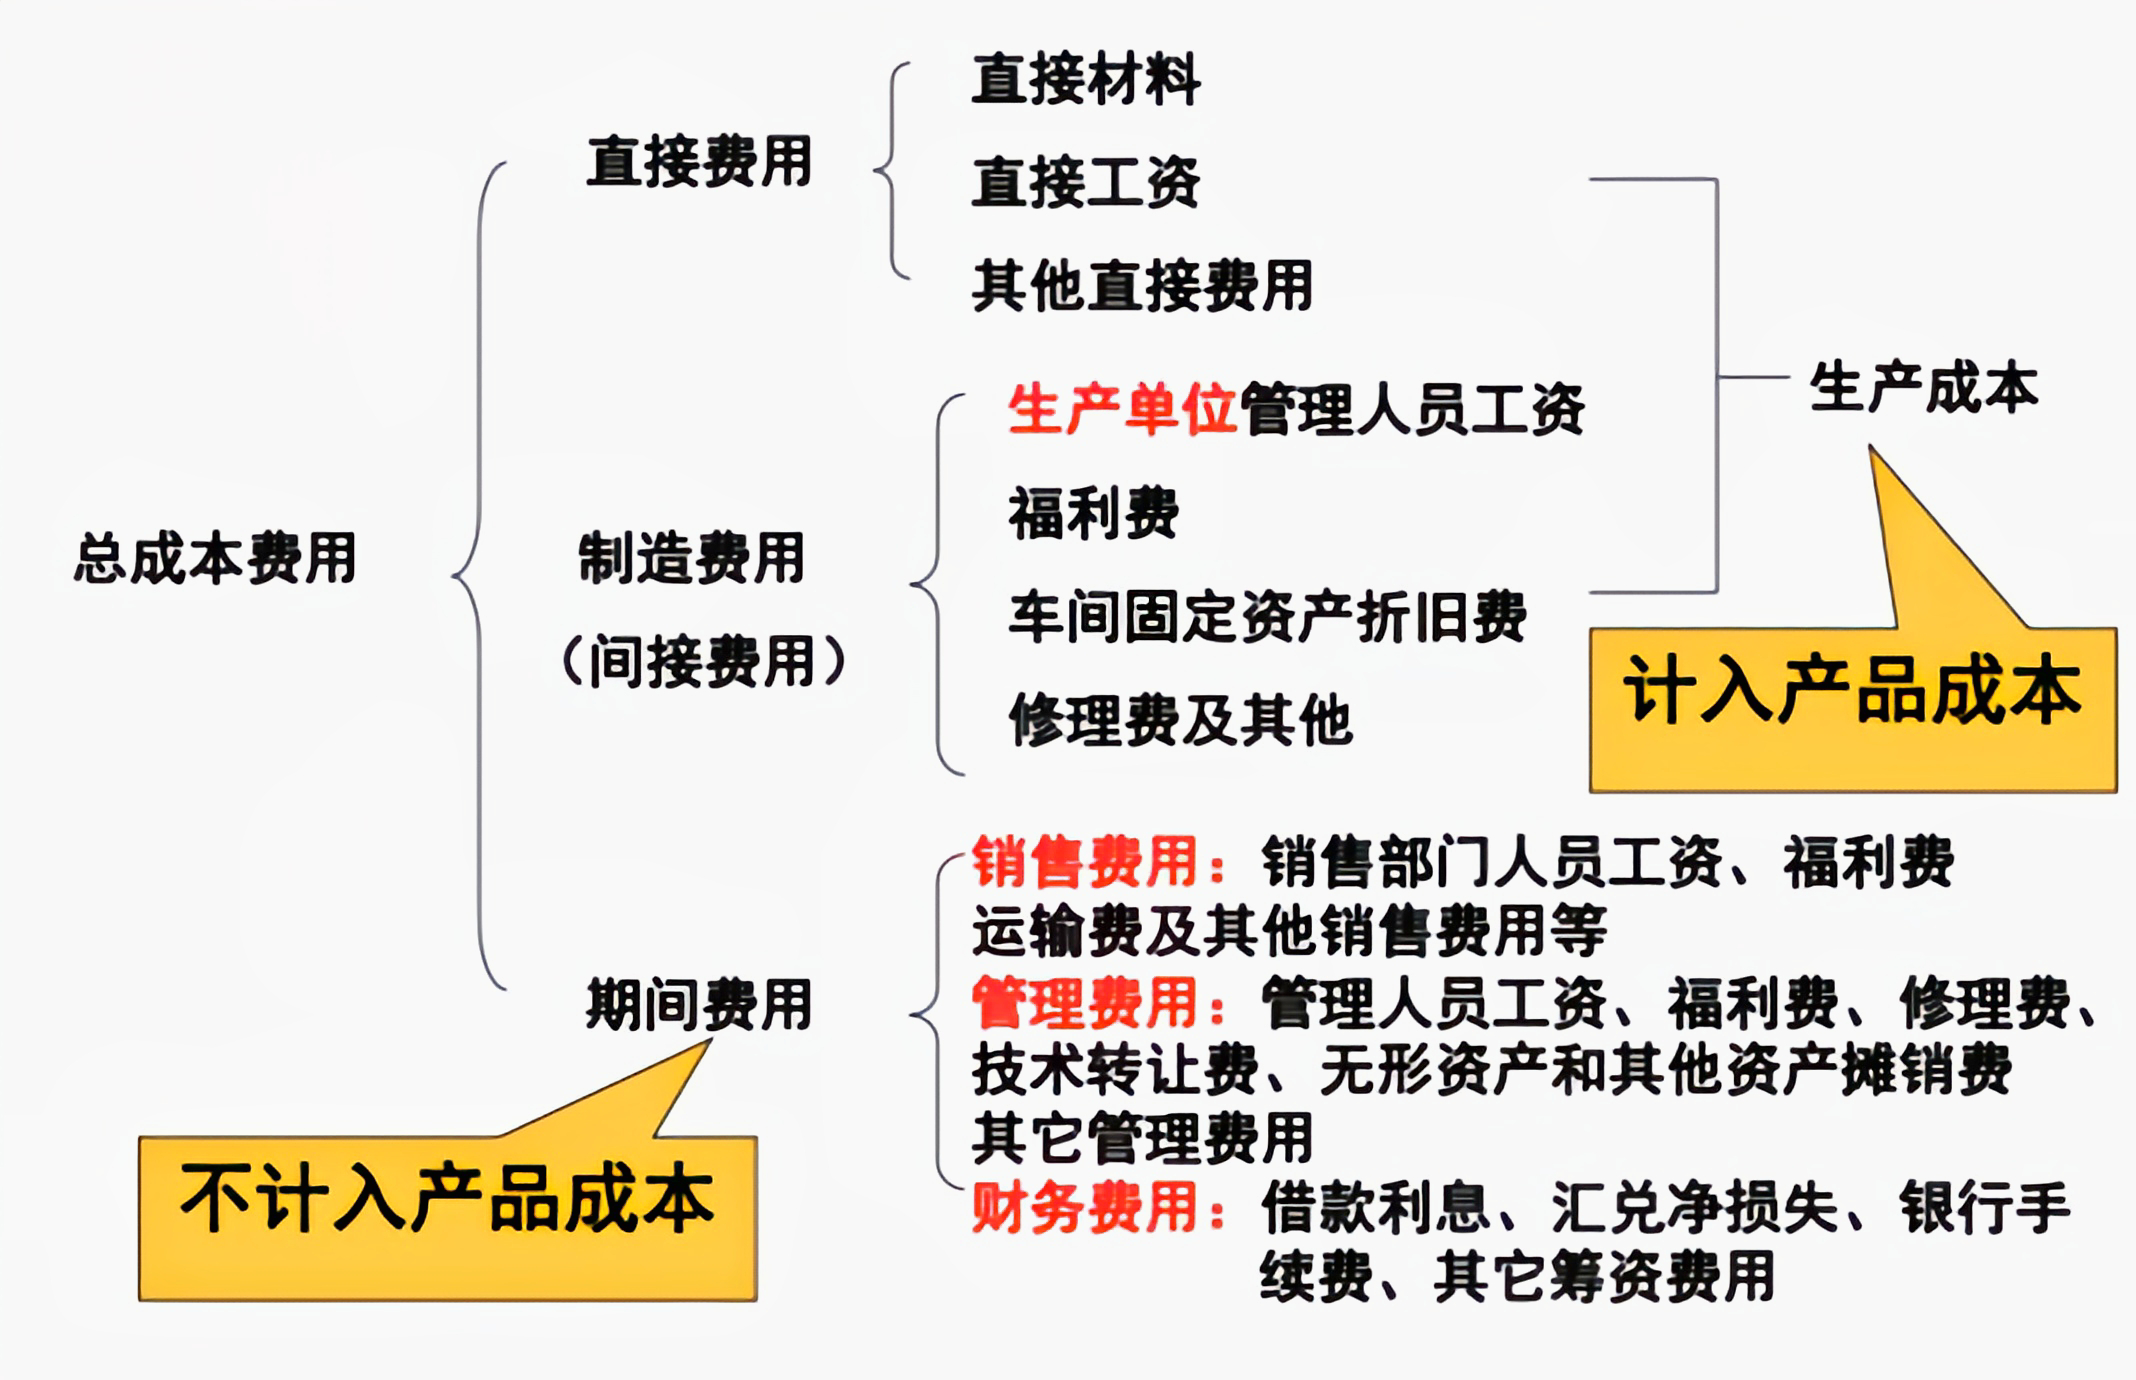
\includegraphics[width=\textwidth]{image/总成本费用构成.png}
    \caption{总成本费用构成图}
\end{figure}

\textbf{(1)直接费用}

直接材料:用于产品生产、构成产品实体的材料的消耗;

直接工资:生产产品的工人工资;

其他直接费用:生产产品的工人福利费、产品生产过程中燃料动力的消耗。

\textbf{(2)制造费用(间接费用)}

界定:生产单位为组织和管理生产所发生的各项间接费用;

举例:生产单位(车间或分厂)管理人员工资、福利生产单位固定资产折旧费、修理费,及其他制造费用(办公、差旅、劳保费等);

直接费用和相应的制造费用,称为产品生产成本;

已销售产品的生产成本,称为产品销售成本。

\textbf{(3)期间费用(不计入产品成本的费用)}

销售费用:商品销售过程中发生的费用,运输、装卸、包装、保险、广告宣传费、专设销售机构的费用等。

管理费用:企业行政管理部门为管理和组织经营活动而发生的各项费用。如管理部门人员工资及福利、折旧、无形资产的摊销、办公费、修理费等;

财务费用:企业在筹集资金等财务活动中发生的费用,包括利息支出、汇兑净损失、银行手续费等。

\subsection{总成本费用构成-按表现形态分类(看看,有个印象就行)}
按照表现形态分类,总成本费用包括:外购材料(原材料、辅料、半成品、包装物、备件、低耗品等)、外购燃料、外购动力、工资+福利费、折旧费、摊销费、利息支出、修理、其他(税金)。

\subsection{技术经济分析中有关成本费用的概念}
(1)技术经济分析中对成本、费用的理解与企业财务会计中的理解不完全相同:

(2)会计中的成本和费用是对企业生产经营过程中实际已经发生的各种耗费的真实、唯一的记录;

(3)技术经济分析中使用的成本和费用数据是在一定假设前提下对拟实施投资方案的未来情况预测的结果,带有不确定性;

(4)会计中对费用和成本的计量是分别针对特定会计期间和特定产品生产过程;

(5)技术经济分析中对费用和成本的计量则一般是针对某一投资项目或技术方案的实施结果;

(6)技术经济对成本、费用的分析,强调对现金流量的影响分析,一般不严格区分成本、费用概念;

(7)技术经济分析中还需引入会计中不使用的一些成本概念。

\textbf{例1:}(判断题)技术经济分析中使用的成本和费用数据是企业生产经营过程中实际已经发生的各种耗费的真实、唯一的记录。

\textbf{答案:}错误。

\textbf{例2:}某公司拟新建车间,需要使用公司现在拥有的一块土地,在进行投资分析时,因为公司不必动用资金去购置土地,应该将该土地的成本考虑在内吗?

\textbf{答案:}应该考虑,这属于\textbf{机会成本}。以下是具体解析。

土地的成本应考虑在内,因为该公司若不利用这块土地兴建车间,则它可将这块土地移作他用,并取得一定的收入。只是现在由于在这块土地上兴建车间才放弃了这笔收入,而这笔收入代表兴建车间使用土地的机会成本。

假设这块土地出售可净得15万元(假设此为该土地所有可能获取收益中最高的收益),它就是兴建车间的机会成本。

Tips:不管该公司当初是以5万元还是20万元购进这块土地,都应以现行市价作为这块土地的机会成本。

\subsection{机会成本}
上个例题引入了一个新的概念,机会成本。这个是需要理解并掌握的。

\subsubsection{涵义:}
机会成本是指将一种具有多种用途的有限资源置于某种特定的用途,而放弃的用于其他各种用途的最高收益。

机会成本的概念来源于这样的现实:资源是稀缺的。资源的稀缺性决定了人类只有充分考虑了某种资源用于其他用途的潜在收益后,才能作出正确的决策使有限的资源得到最佳、有效的利用。

\subsubsection{意义:}
机会成本不是一种实际发生的支出或费用,而是失去的收益,这种收益不是实际发生的,而是潜在的。\textbf{它在会计记录中是没有的。}

在决策中,机会成本有利于人们全面考虑可能采取的各种方案,以便为特定、稀缺资源寻求最为有利的使用途径。在技术经济分析中,\textbf{机会成本会影响现金流量。}

\textbf{例1:}企业有一台机多用床,可以自用,也可以出租,出租可以获得7000元的年净收益,自用可以产生6000元的年净收益。

1. 当舍弃出租方案而采用自用方案时,其机会成本为 [填空1] ,其利益为 [填空2] ;

2. 当舍弃自用方案而采用出租方案时,其机会成本为 [填空3] ,利益为 [填空4] 。

\textbf{答案:}7000元;-1000元;6000元;1000元。

\textbf{例2:}某公司在2017年曾经打算新建一个车间,并请一家公司作过可行性分析,支付咨询费5万元。后来由于各种原因该项目被搁置下来。 2019年旧事重提,在进行投资分析时,这笔咨询费是否需要考虑呢?

\textbf{答案:}不需要。这属于\textbf{沉没成本}。无论是否进行投资,这笔支出都不会改变。

\subsection{沉没成本}
那么上题就引入了新概念,沉没成本。需要理解,但不是重点。
\subsubsection{涵义:}
沉没成本是指过去已经支出的,与当前决策无关的成本。
\subsubsection{意义:}
它对企业决策不起作用,它主要表现为过去发生的事情,费用已经支付,今后的任何决策都不能取消这项支出。

如果将沉没成本纳入投资方案的总成本,则一个有利的方案可能因此变得不利,从而造成决策错误。\\
\textbf{例题:}(单选)在项目投资中,下列哪一个因素不应该考虑\\
A. 现金流入\\
B. 机会成本\\
C. 沉没成本\\
D. 资金成本\\
\textbf{答案:}C。

\subsection{经营成本/付现成本}
此部分需要\textbf{理解并掌握}。

\subsubsection{引入:}
在技术经济分析中,需要考察投资项目的现金流入与现金流出。按照会计核算的方法,总成本费用中含有既不属于现金流入也不属于现金流出的\textbf{折旧和摊销费}。

建设投资中有固定资产投资和无形资产投资部分,已作为现金流出,总成本费用中又有对固定资产和无形资产的按期计提的折旧和摊销,若再作为流出,等于多流出一次,故要计算项目各年实际发生的现金流出,\textbf{必须从总成本费用中将折旧费和摊销费剔除。}

\textbf{即经营成本是为了经济分析方便,从总成本费用中分离出来的与投资分摊、资金筹措无关的一部分费用。}

计算:

经营成本=总成本费用-折旧费-摊销费-\textbf{借款利息支出}

注意:

技术经济分析中通常将“经营成本”作为一个单独的现金流出项;

如果分析中需要考虑借款利息支出,则另列一个现金流出项。

\noindent \textbf{例题:}(多选)下列说法错误的是\\
A. 机会成本任何时候都不影响现金流量\\
B. 经营成本是现金流出\\
C. 总成本费用是现金流出\\
D. 沉没成本不影响项目未来的现金流\\
\textbf{答案:}AC。

\section{营业收入}
\textbf{涵义:}通过销售产品、提供劳务等取得的货币收入。

\textbf{作用:}是技术经济分析中现金流入的重要组成部分;

\textbf{计算:}销售收入=商品销量 × 商品销售单价(以市场价格计算)

\section{税金}
\subsection{概念(了解即可)}
税收:国家为了实现其职能、凭借政治权力,按法律规定的标准,强制地、无偿地取得财政收入的一种特定的分配形式。

税金:国家依据法律对有纳税义务的单位和个人征收的财政资金。

作用:积累财政资金,进行宏观调控。

\textbf{税金和费用的区别:}
费用是政府机关为单位或居民个人提供服务或授予国家资源和资金的使用权而收取的代价,遵循\textbf{有偿}原则。

\subsection{税金的分类-按性质和作用分类(了解)}
\textbf{(1)流转税类:}

以商品生产、流通和劳动服务的流转额为征税对象。

内容:增值税、消费税。

\textbf{(2)所得税类:}

以法人或个人的纯所得为征税对象的各种税。

内容:企业所得税、个人所得税。

\textbf{(3)资源税类:}

以被开发或占用的资源为征税对象的各种税。

内容:资源税、土地使用税。

\textbf{(4)财产税类:}

以法人或自然人拥有及转移的财产价值或增值额为征税对象的各种税。

内容:房产税、车船使用税、土地增值税。

\textbf{(5)特定目的税类:}

国家为达到某种特定目的而设立的各种税。

内容:城市维护建设税、车辆购置税、印花税等。

\textbf{(6)关税}

主要对进出我国国境的货物、物品征收。

内容:关税。

\subsection{主要税种的涵义、纳税金额的计算}
重点:\textbf{增值税}、消费税、城市维护建设税、教育费附加、\textbf{企业所得税}等。

\subsubsection{(1)增值税}
\textbf{征收对象:}增值税是对在我国境内销售货物或提供加工、修理修配劳务以及进口货物的单位和个人征收的一种税。\textbf{增值税是价外税。}增值税不影响最后利润。

\textbf{应纳税额的计算(一般纳税人)}

计算公式为:

应纳税额=当期销项税额-当期进项税额

销项税额=销售额(销售时销售方收取)×增值税税率(0,6\%,9\%,13\%)

进项税额=购买价款(购买时购买方支付)×增值税税率(0,6\%,9\%,13\%)

\textbf{增值税的流程:}
\begin{figure}[H]
    \centering
    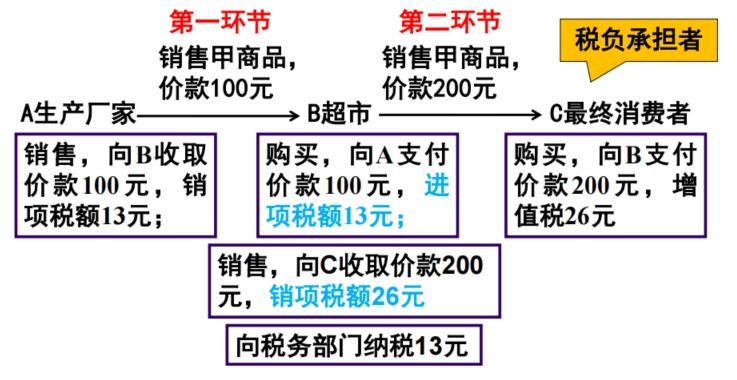
\includegraphics[width=\textwidth]{image/增值税流程图.png}
    \caption{增值税流程图}
\end{figure}

\textbf{例题:}某超市某月购进一批商品,商品应税进价100,000元,当月销售该批商品,应税销售总金额150,000元,增值税税率为13\%,计算该超市在当月应缴纳的增值税为[填空1]。\\
答案:$(150000-100000) \times 13\% = 6500$(元)

\textbf{注意:}

要回答这个题,首先要知道什么是“应税”。应税,通俗来讲,就是应该交税,但实际还没交。因此这里是不含税价格。

当纳税人销售货物和应税劳务采用含税价格(销售额和销项税额合并定价方法)时,按下列公式计算销售额:

销售额=含税销售额$\div$(1+税率)

目测大小案例分析时有应用。\\
\textbf{例题:}某拟建工业项目,根据产品生产方案,计划在达产期每年需购进应税原料价款2040.2万元,增值税税率13\%;年计划销售自产产品1万吨,含税销售额为2950万元,增值税税率13\%。试计算该企业建成达产后预计应纳增值税税额是多少?\\
A. 339.38\\
B. 265.23\\
C. 74.15\\
D. 66.83\\
\textbf{答案:}C。解析如下。

根据一般纳税人应纳增值税计算方法,分三步计算。

第一步计算应税销售额:

应税销售额$=2950/1.13=2610.62$(万元)

第二步计算销项与进项税额:

销项税额$=2610.62×13\%=339.38$(万元)

进项税额$=2040.2×13\%=265.23$(万元)

第三步计算应纳税税额:

应纳增值税税额$=339.38-265.23=74.15$(万元)

即该企业在达产期各年预计应纳增值税税额74.15万元。

\noindent \textbf{增值税对现金流量的影响}

增值税为\textbf{价外税},当采用不含(增值)税价格计算销售收入、原材料、燃料动力时,利润表和利润分配表以及现金流量表中不包括增值税科目。也即可以\textbf{不考虑增值税}。

当采用含(增值)税价格计算时,利润表和利润分配表以及现金流量表中应单列增值税科目。

\noindent \textbf{增值税的处理}

\noindent \textbf{不含税}

现金流入:销售收入 200(不含税)

现金流出:购进原材料部分 100

\noindent \textbf{含税}

现金流入:销售收入 $226(200+200 \times 13\%)$(含税)

现金流出:购进原材料部分 $113(100+100 \times 13\%)$;
增值税 13

\subsubsection{(2)消费税(了解即可)}
\textbf{征税范围}

消费税是对在我国境内生产、委托加工和进口国家规定的应税消费品的单位和个人征收的一种流转税。

\textbf{应税消费品:}烟、酒及酒精、化妆品、贵重首饰及珠宝玉石、鞭炮烟火、汽油、柴油、汽车轮胎、摩托车、小汽车;

\textbf{应纳税额的计算}

其一,从价定率:消费品应纳税额=应税消费品销售额×消费税税率

其二,从量定额:消费品应纳税额=应税消费品的数量×单位税额

\subsubsection{(3)城市维护建设税(上机案例分析会应用)}
\textbf{征税范围}

城市维护建设税是国家对缴纳增值税、消费税的单位和个人就其实际缴纳的“三税”税额为计税依据而征收的一种税。其税款用于城市公用事业和公共设施维护建设。

\textbf{应纳税额的计算}

城市维护建设税=纳税人实际缴纳的两税×地区适用税率

\textbf{税率:}
市区:7\%;
县城、镇:5\%;
不在市区、县城或镇:1\%。
\subsubsection{(4)教育费附加(上机案例分析会应用)}
\textbf{征收范围}

对缴纳增值税、消费税的单位和个人,就其实际缴纳的“两税”税额为计算依据而征收的一种附加费。

\textbf{计算}

教育费附加=纳税人实际缴纳的两税×税率(3\%)

\subsubsection{(5)企业所得税(上机案例分析会应用,掌握计算)}
\textbf{征税范围}

国家对境内企业生产、经营所得和其他所得征收的一种税。

\textbf{应纳税额的计算}

应纳税额=应纳税所得额×税率(25\%)

\textbf{技术经济中简化运用}

应纳税额=利润总额×税率

\noindent \textbf{例题:}某设备总价1000万元,预计设备残值率为5\%,设备当年用于生产,生产期采用直线折旧法折旧,折旧年限5年,预计年销售收入1000万元,年经营成本500万元,年营业税金及附加80万元。所得税税率25\%,生产期内每年的企业所得税是多少?
\begin{figure}[H]
    \centering
    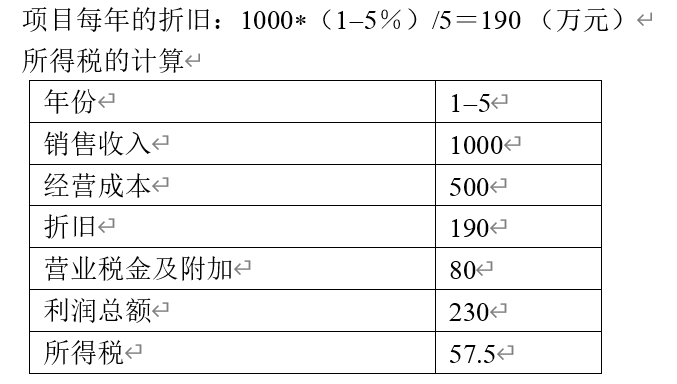
\includegraphics[width=0.8\linewidth]{image/税金-企业所得税.png}
\end{figure}

\subsubsection{总结}
总结:各种税金的计入方向、对现金流的影响(上机时会用到)

(1)增值税当不含税价格时,不考虑,含税价格时单列;

(2)消费税、城市维护建设税、资源税、教育费附加等计入营业税金及附加为现金流出,同时在计算利润时从收入中扣除;

(3)所得税从利润总额中征收,计入所得税,为一项现金流出。

\noindent 考察例题:

\noindent \textbf{例1:}(多选)下列说法错误的是\\
A.机会成本任何时候都不影响现金流量\\
B.经营成本是现金流出\\
C.总成本费用是现金流出\\
D.沉没成本影响项目未来的现金流\\
E.流动资金投资是现金流出\\
\textbf{例2:}(判断题)经营成本=总成本费用-折旧费-摊销费+借款利息支出。\\
\textbf{例3:}(判断题)增值税是价外税。\\
\textbf{答案:ACD;错误;正确。}

\subsection{利润(要求理解并掌握)}
销售利润=销售收入-产品销售成本-产品营业(销售)税金及附加-销售费用-管理费用-财务费用

即销售利润=销售收入-总成本费用-产品营业(销售)税金及附加

税后利润(净利润)=销售利润-所得税

\noindent \textbf{例1:}某项目固定资产原值1000万元,预计固定资产净残值率为5\%,生产期第一年开始按照直线折旧法折旧,折旧年限10年,预计年销售收入1000万元,年经营成本600万元,年营业税金及附加100万元。生产期内每年的利润总额为多少?\\
答:
\begin{figure}[H]
    \centering
    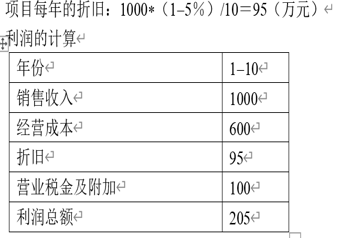
\includegraphics[width=0.8\linewidth]{image/利润总额.png}
\end{figure}
\begin{figure}[H]
    \centering
    \caption{销售收入、成本、税金和利润关系图}
    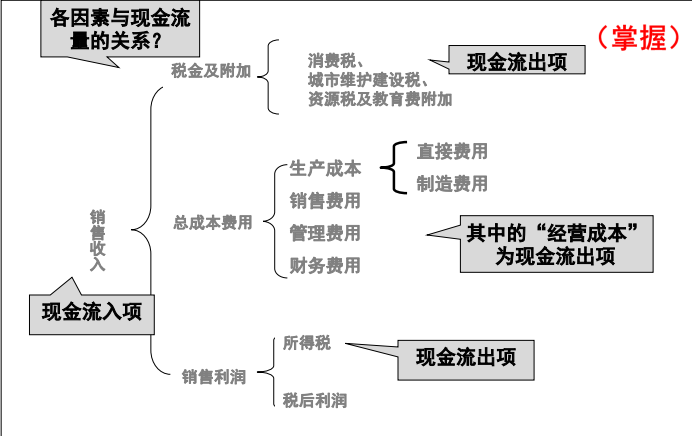
\includegraphics[width=0.8\linewidth]{image/销售收入、成本、税金和利润关系图.png}
\end{figure}
\noindent \textbf{例2:}(多选)以下为现金流出项的为:\\
A.所得税;B.经营成本;C.销售收入;D.城市维护建设税\\
\textbf{答案:}ABD。

\section{按期间构成的项目现金流量}

现金流量的构成与计算:初始现金流量(Initial Cash Flow)、营业现金流量(Operating Cash Flows)、终结现金流量(Terminal Cash Flow)。

\begin{figure}[H]
    \centering
    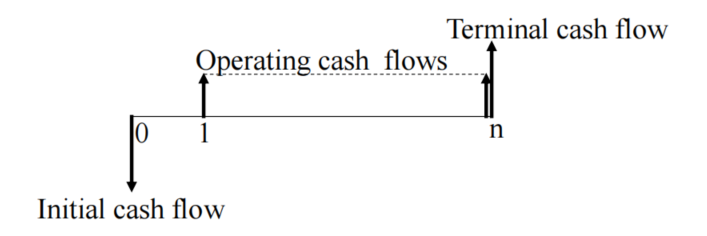
\includegraphics[width=0.8\linewidth]{image/现金流量的构成.png}
    \caption{现金流量的构成}
\end{figure}

\subsection{初始现金流量}
\subsubsection{(1)固定资产投资}
固定资产的购置成本或建造费用,以及运输费、安装费等。
\subsubsection{(2)流动资金投资}
即流动资金,包括对原材料、在产品、产成品和现金等方面的投资。
\subsubsection{(3)其他投资费用}
如职工培训费、谈判费、注册费等开办费。
\subsubsection{(4)原有固定资产变价的税后净收入(设备更新决策)}


\subsection{营业现金流量}
\subsubsection{(1)营业收入}
\subsubsection{(2)税金及附加}
\subsubsection{(3)经营成本}
\noindent 经营成本=总成本费用-折旧和摊销-利息
\subsubsection{(4)所得税}
\subsubsection{(5)计算}
\noindent 营业净现金流量\\
=营业收入-经营成本-税金及附加-所得税\\
=营业收入-(总成本费用-折旧/摊销-利息)-税金及附加-所得税\\
=营业收入-总成本费用-税金及附加-所得税+折旧/摊销+利息\\
=销售利润-所得税+折旧、摊销+利息\\
=税后利润+折旧、摊销+利息

\subsection{终结现金流量}
\subsubsection{(1)固定资产预计净残值}
\subsubsection{(2)流动资金投资回收}

\section{现金流量图}
\subsection{含义}
现金流量图是表示项目系统在整个寿命周期内各时间点的现金流入和现金流出状况的一种图示。

\subsection{绘法}
(1)以横轴为时间坐标,时间间隔相等,时间轴上的点称为时点,时点表示该期的期末,同时也是下一期的期初,零时点即为第一期开始之时点。

(2)以纵轴为现金流量坐标,单位可取元、或万元。

(3)与横轴相连的垂直线,箭头向上表示现金流入,向下表示现金流出,长短与现金流量绝对值的大小成比例,箭头处一般应标明金额。

$\downarrow$ 表示现金流出:某一个时间点的流出系统的固定资产投资;流动资金投资;经营成本;销售税金及附加;所得税。

$\uparrow$ 表示现金流入:某一个时间点的流入系统的资金销售收入;固定资产残值回收;流动资金回收

同一个时间点的现金流入与现金流出的差额叫净现金流量。

系统的现金流入、现金流出和净现金流量统称为现金流量。

一般情况,时间单位为年,假设投资发生在年初,销售收入、经营成本及残值回收等均发生在年末。
$$
\mbox{固定资产净值 = 固定资产原值 - 累计折旧}
$$

期末残值:项目寿命期结束时固定资产的残余价值。

\subsection{现金流量图的进一步说明}
时点:时间坐标的原点通常取在建设期开始的时点,也可取在投产期开始点,而分析计算的起始时间一般都规定在时间坐标的原点。

为了统一绘制方法和便于比较,通常规定投资发生在各时期的期初,而销售收入、经营成本、利润、税金等,则发生在各个时期的期末,回收固定资产净残值与回收流动资金在项目经济寿命周期终了时发生。

第t时点,既表示是第t期末,也表示是第t+1期初。

\textbf{例1:}某工程投资为120万元,一年投产。年销售收入为100万元,年折旧费为20万元,计算期n为6年,固定资产残值为零,年经营成本为50万元,所得税税率为25\%。试求年净现金流量并画出现金流量图。

\textbf{解:}令A为该项目投产后年净现金流量,则:

初始现金流量=-120

营业年现金流量=税后利润+折旧

税后利润=年收入-年总成本费用-年所得税$=(100-50-20)-(100-50-20) \times 25\%=22.5$万元

营业年现金流量$=22.5+20=42.5$万元

现金流量图:
\begin{figure}[H]
    \centering
    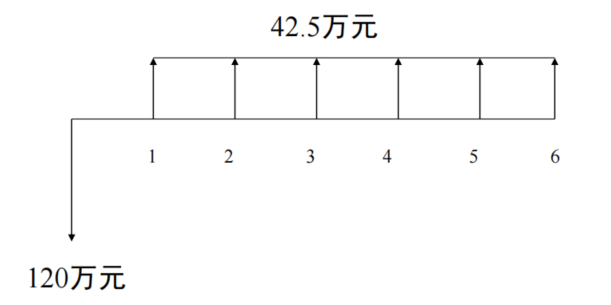
\includegraphics[width=0.75\linewidth]{image/现金流量图-例题.png}
\end{figure}

\textbf{例2:}有一投资项目,固定资产投资50万元,流动资金投资20万元,均于第1年年初投入。项目当年建成投产,产品销售第1年为50万元,第2-7年为80万元;经营成本第1年为30万元,第2-7年为45万元;第1-7年折旧费每年为6万元,第7年末处置固定资产可得收入8万元,所得税税率为25\%。编制该项目的现金流量表。

\begin{figure}[H]
    \centering
    \caption{项目生产期各年的(调整)所得税:}
    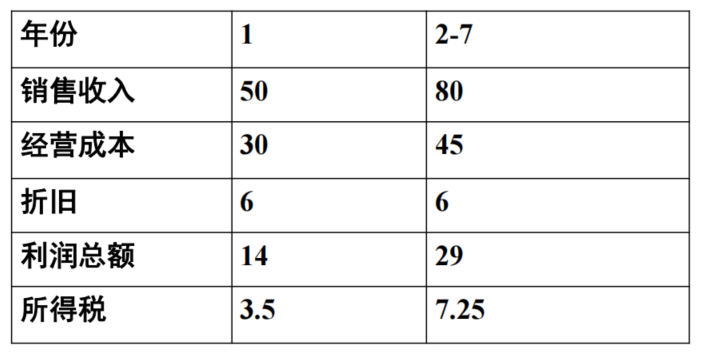
\includegraphics[width=0.75\linewidth]{image/项目生产期各年的(调整)所得税.png}
\end{figure}

\begin{figure}[H]
    \centering
    \caption{项目投资现金流量表}
    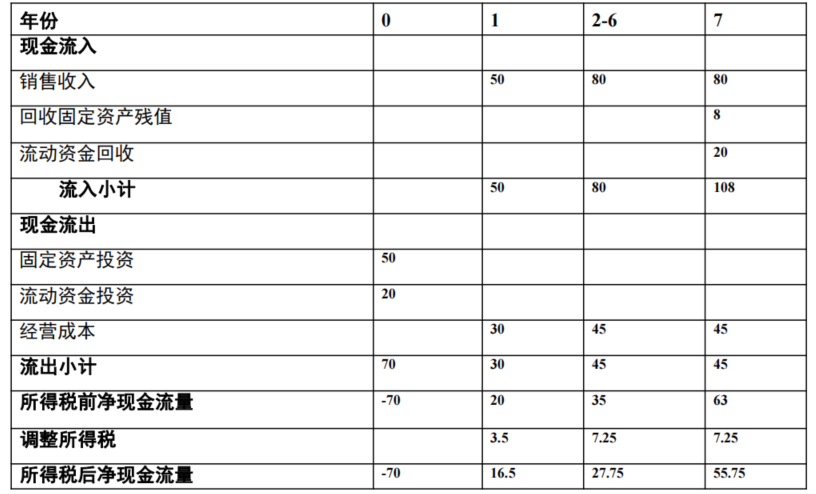
\includegraphics[width=\linewidth]{image/项目投资现金流量表.png}
\end{figure}

\section{现金流量表}
\begin{figure}[H]
    \centering
    \caption{现金流量表}
    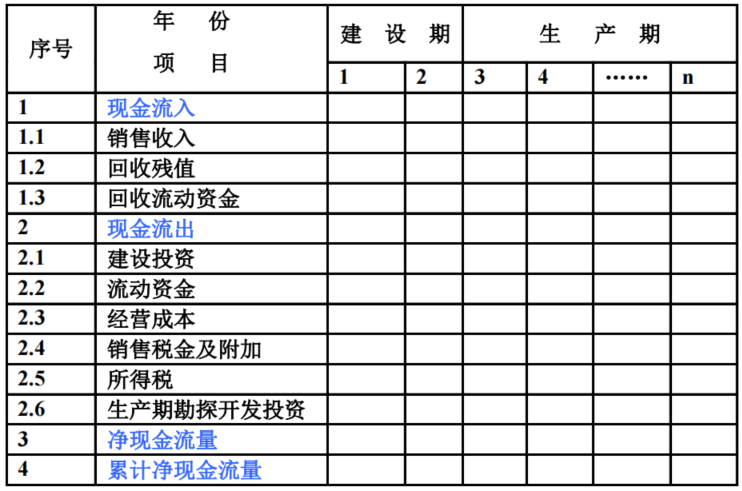
\includegraphics[width=1\linewidth]{image/现金流量表.png}
\end{figure}

\section{分析现金流量应注意的问题(需要理解掌握)}
\noindent \textbf{注意折旧对所得税的影响}

折旧不是现金流出,但不同的折旧方法将影响企业税前利润的计算,从而影响企业的所得税支出,影响现金流量。

\noindent \textbf{沉没成本不是现金流:}以往发生的与当前经营决策无关的成本。
\noindent \textbf{考虑机会成本的影响}

当一种资源用于多种用途时所放弃的其他投资机会中最佳的投资机会。

\noindent \textbf{注意流动资金的投入和收回}

\noindent \textbf{注意财务成本}

例:(多选)下列费用中()不是现金流量\\
A.原材料\\
B.折旧\\
C.沉没成本\\
D.管理费用\\
答案:BC。

\section{总结}
\noindent \textbf{本节重点}\\
1、总投资的两大构成\\
2、固定资产的各种计价\\
3、固定资产折旧方法(直线法)\\
4、对折旧、摊销的理解\\
5、会计和技术经济中成本费用的区别\\
6、技术经济中的四种成本\\
7、各种税对现金流量的影响\\
8、营业收入、成本、税金和利润关系图

\textbf{思考题1:}承德某饮品企业L和江苏某IT企业J均为上市公司,2000年的年报数据表明这两家公司有良好的业绩表现,但L企业采用直线折旧法折旧,而J企业采用加速折旧法,分析这两家企业的发展策略。

\textbf{思考题2:}某公司固定资产投资为5万元,该资产有效期为3年,不考虑折旧前提下,该公司所产生的营业利润为:第一年2万元,第二年3万元,第三年2.5万元。该项目的流动资金为1.5万元。该项目的现金流是多少?

\textbf{思考题3:}某企业购入一项原价24300元的固定资产,估计残值为300元,使用寿命期为4年,试用直线折旧和双倍余额折旧方法分别计算每年的折旧额,累计折旧额和账面资产净值。